\documentclass[a4paper, 12pt]{article}

\usepackage[T2A]{fontenc}
\usepackage[utf8]{inputenc}
\usepackage[english,russian]{babel}
\usepackage[left=15mm, top=20mm, right=15mm, bottom=20mm, nohead, nofoot]{geometry}

\usepackage{hyperref}
\usepackage{graphicx}
\usepackage{wrapfig}
\usepackage{afterpage}
\usepackage{amsmath, amsfonts, amssymb, amsthm, mathtools}
\author{Волос Полина, группа Б06-907}
\title{ВПВ по курсу "Электричество и магнетизм" \\ Конденсатор на высоких частотах}
\date{28 декабря 2021 г.}
%%%%%%%%%%%%%%%%%%%%%%%%%%%%%%%%%%%%%%%%%%%%%%%%%%%%%%%%%%%%%%%%%%%%%%%%%
\usepackage{graphicx, wrapfig, subcaption, setspace, booktabs}
\usepackage[protrusion=true, expansion=true]{microtype}
\usepackage[english]{babel}
\usepackage{sectsty}
\usepackage{url, lipsum}
\newcommand{\HRule}[1]{\rule{\linewidth}{#1}}
\onehalfspacing
\setcounter{tocdepth}{5}
\setcounter{secnumdepth}{5}
%%%%%%%%%%%%%%%%%%%%%%%%%%%%%%%%%%%%%%%%%%%%%%%%%%%%%%%%%%%%%%%%%%%%%%%%%


\begin{document}

\title{ \normalsize \textsc{ВОПРОС ПО ВЫБОРУ}
		\\ [4.0cm]
		\HRule{0.5pt} \\ [0.3cm]
		\LARGE \textbf{{КОНДЕНСАТОР НА ВЫСОКИХ ЧАСТОТАХ}}
		\HRule{0.5pt} \\ [0.1cm]
		\normalsize  \vspace*{20\baselineskip}}

\date{}

\author{
		Хомутов Андрей, Б06-903 \\
ФБМФ, 2020\\ }

\maketitle
\thispagestyle{empty}
\newpage

$\huge{\text{П}}$редставим, \textbf{\text{что}} к обкладкам конденсатора приложено напряжение низкой частоты. Тогда без учета краевых эффектов однородное поле внутри конденсатора может быть представлено как
\begin{equation}E=E_{0} e^{i \omega t}.\end{equation}

Пусть теперь изменение поля достаточно быстро, учтем появление магнитного поля с помощью одного из уравнений Максвелла:
\begin{equation} \oint_{\Gamma} (\boldsymbol{B} \cdot d \boldsymbol{l})=\frac{1}{c}\frac{d}{d t} \int_{S} (\boldsymbol{E} \cdot d\boldsymbol{S}).\end{equation}
Взяв в качестве кривой $\Gamma_{1}$ кольцо радиуса $r$, получим:
\begin{equation}c^{} B \cdot 2 \pi r=\frac{\partial}{\partial t} E \cdot \pi r^{2}.\end{equation}
А с учетом (1) в нашем конденсаторе магнитное поле равно
\begin{equation}B=\frac{i \omega r}{2 c} E_{0} e^{i \omega t}.\end{equation}

\begin{figure}[h]
    \begin{center}
    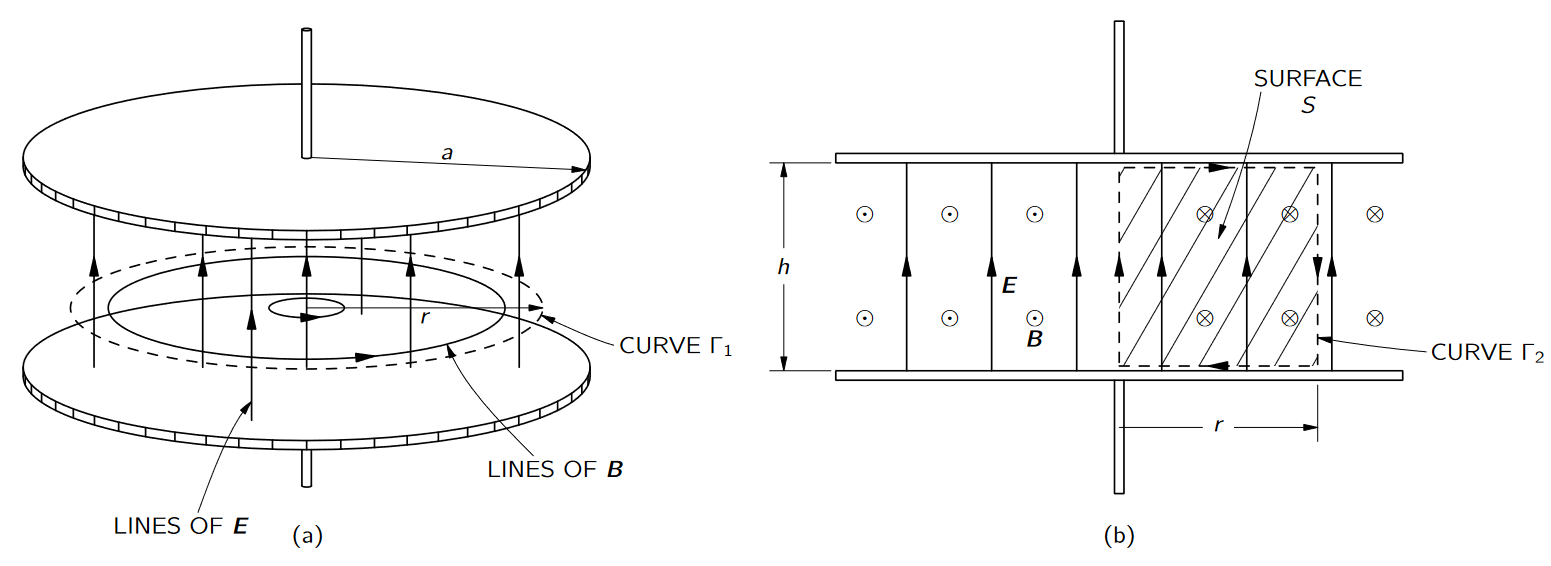
\includegraphics[width=1\textwidth]{capasitor.png}
    \end{center}
    \caption{$\boldsymbol{E}$ и $\boldsymbol{B}$ между обкладок конденсатора}
\end{figure}

Но изменяющееся магнитное поле согласно другому уравнению Максвелла приведет к появлению вихревого электрического поля. При этом, как мы видим, с ростом частоты растет магнитное поле, так как оно пропорционально скорости изменения электрического, и импеданс конденсатора уже не будет выражаться как $1 / i \omega C$. Так, с ростом частоты электрическое поле утратит свою однородность.

Попробуем найти правильное электрическое поле, введя поправку к тому полю что было на низких частотах. Тогда, обозначив поле из выражения (1) за $E_{1}$, запишем поле в виде:
\begin{displaymath}E=E_{1}+E_{2},\end{displaymath}
\newpage
где $E_{2}$ - поправка из-за переменного магнитного поля. Для всех частот будем выбирать $E_{0}$ так, чтобы в центре поправки не было ($E_{2} = 0$ при $r = 0$).

Чтобы найти $E_{2}$ воспользуемся уравнением Максвелла уже для циркуляции электрического поля
\begin{equation}\oint_{\Gamma} (\boldsymbol{E} \cdot d \boldsymbol{l})=-\frac{1}{c}\frac{d}{d t} \int_{S} (\boldsymbol{B} \cdot d\boldsymbol{S}).\end{equation}
Взяв в качестве кривой $\Gamma_{2}$ прямоугольный контур, одна из сторон которого расположена на оси, а две перпендикулярных ей проходят по радиусу вдоль обкладок (рис. 1 (b)), то циркуляцию посчитать несложно. Она будет равна $-E_{2}(r) \cdot h$, где $h$ - расстояние между обкладок конденсатора (полагая $E_{2}$ положительным, когда оно направлено вверх). Тогда $E_{2}$ можно найти как
\begin{equation}E_{2}(r)=\frac{1}{c}\frac{\partial}{\partial t} \int B(r) d r.\end{equation}

Используя (4) для $B(r)$ получаем
\begin{displaymath}E_{2}(r)=\frac{\partial}{\partial t} \frac{i \omega r^{2}}{4 c^{2}} E_{0} e^{i \omega t}.\end{displaymath}
После дифференцирования просто добавляется еще один множитель $i\omega$:
\begin{equation}E_{2}(r)=-\frac{\omega^{2} r^{2}}{4 c^{2}} E_{0} e^{i \omega t}.\end{equation}
Ожидаемо, что поправочное поле имеет направление противоположное основному. Таким образом, исправленное поле будет равно
\begin{equation}E=E_{1}+E_{2}=\left(1-\frac{1}{4} \frac{\omega^{2} r^{2}}{c^{2}}\right) E_{0} e^{i \omega t}.\end{equation}
Электрическое поле уже не будет однородно, теперь оно имеет параболическую форму (штриховая линия на рис. 2).
\begin{figure}[h]
    \begin{center}
    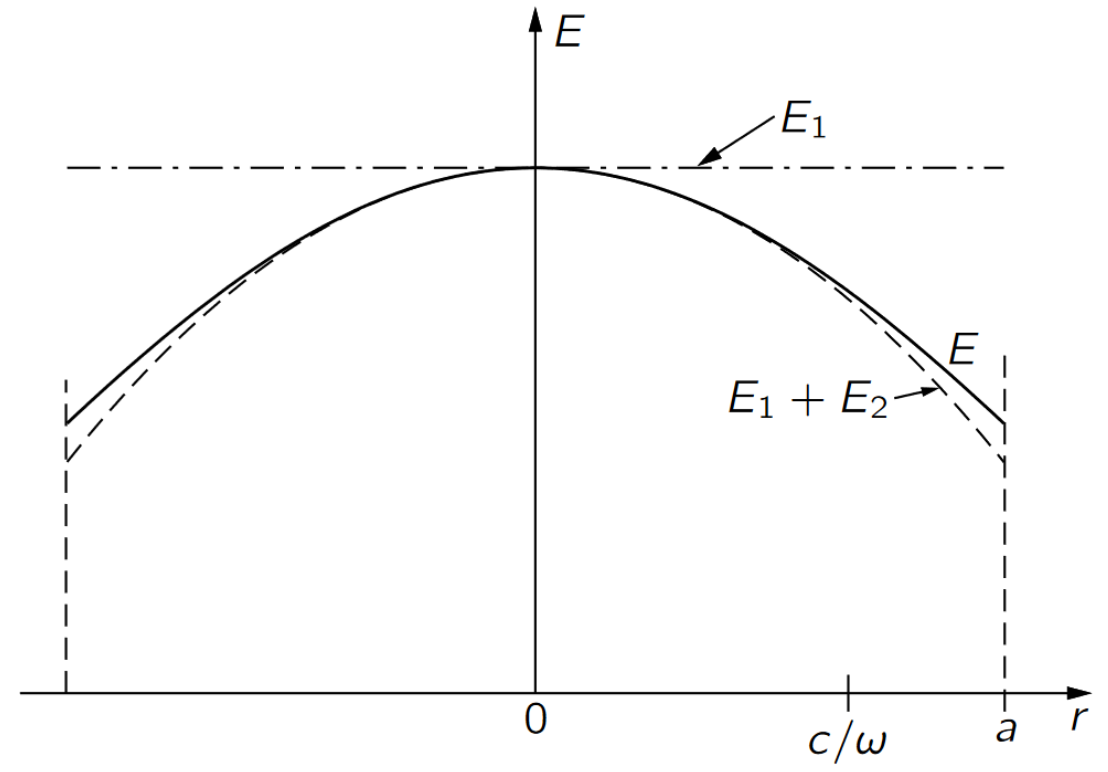
\includegraphics[width=0.5\textwidth]{feild.png}
    \end{center}
    \caption{$\boldsymbol{E}$ между обкладок на высоких частотах (без учета краевых эффектов)}
\end{figure}


Продолжим наши рассуждения. Так как мы учли добавочное поле $E_{2}$, появляющееся из-за изменяющегося магнитного, можно учесть то, что само поле $B$ уже не будет прежним. Проведем аналогичные операции и разобьем поле $B_{1}$ равное (4) и $B_{2}$ - поправку из-за учтенного поля $E_{2}$. 

Чтобы найти его, снова воспользуемся уравнением (3):
\begin{displaymath}c^{} B_{2} \cdot 2 \pi r=\frac{1}{c}\frac{d}{d t} \int_{S} (\boldsymbol{E_{2}} \cdot d\boldsymbol{S}).\end{displaymath}
С учетом того, что $E_{2}$ зависит от радиуса
\begin{displaymath}\Phi_{E_{2}}=\int_{0}^{r} E_{2}(r) \cdot 2 \pi r d r.\end{displaymath}
Тогда
\begin{equation}B_{2}(r)=\frac{1}{r c} \frac{\partial}{\partial t} \int E_{2}(r) r d r.\end{equation}
Подставляя $E_{2}(r)$ из (7), получаем интеграл от $r^{3} d r$, и поправка к магнитному полю будет равна
\begin{equation}B_{2}(r)=-\frac{i \omega^{3} r^{3}}{16 c^{3}} E_{0} e^{i \omega t}.\end{equation}
С уточнением формулы для магнитного поля придется снова корректировать выражение для электрического. Снова используя соотношение (6)
\begin{equation}E_{3}(r)=\frac{1}{c}\frac{\partial}{\partial t} \int B_{2}(r) d r\end{equation}
Подставляя сюда результат (10), получим новую поправку к электрическому полю:
\begin{equation}E_{3}(r)=+\frac{\omega^{4} r^{4}}{64 c^{4}} E_{0} e^{i \omega t}.\end{equation}
Тогда если дважды исправленное электрическое поле записать в виде $E=E_{1}+E_{2}+E_{3}$, то получим
\begin{equation}E=E_{0} e^{i \omega t}\left[1-\frac{1}{2^{2}}\left(\frac{\omega r}{c}\right)^{2}+\frac{1}{2^{2} \cdot 4^{2}}\left(\frac{\omega r}{c}\right)^{4}\right].\end{equation}
Получается что изменение электрического поля имеет уже не параболический вид как было раньше, оно лежит чуть выше чем на рис. 2.

Понятно, что новые поправки к $E$ будут вызывать поправки к $B$ и наоборот. Для $B_{3}$ можно использовать (9) с заменой индексов с 2 на 3. Очередная поправка к электрическому полю будет равна
\begin{displaymath}E_{4}=-\frac{1}{2^{2} \cdot 4^{2} \cdot 6^{2}}\left(\frac{\omega r}{c}\right)^{6} E_{0} e^{i \omega t}.\end{displaymath}
Тогда становится понятно рекуррентное соотношение для продолжения ряда
\begin{equation}E=E_{0} e^{i \omega t}\left[1-\frac{1}{(1 !)^{2}}\left(\frac{\omega r}{2 c}\right)^{2}+\frac{1}{(2 !)^{2}}\left(\frac{\omega r}{2 c}\right)^{4}-\frac{1}{(3 !)^{2}}\left(\frac{\omega r}{2 c}\right)^{6} \pm \cdots\right].\end{equation}
Окончательное решение запишем как
\begin{equation}E=E_{0} e^{i \omega t} J_{0} \left(\frac{\omega r}{c}\right).\end{equation}

Здесь, $J_{0}(x)$ - функция Бесселя первого рода 0-го порядка, аргументом которой является $x=\frac{\omega r}{c}$. Реально для расчетов будет достаточно третьего приближения, которое практически совпадает с точным ответом, представленным сплошной линией на рис. 2.





\end{document}